
\documentclass[8pt]{article}

\usepackage[utf8]{inputenc}

\usepackage{amsmath, bm}
\usepackage{graphicx}
\usepackage{amssymb}
\usepackage{float}
\usepackage{caption}
\usepackage{subcaption}
% set font size to 11pt


\setlength{\parskip}{\baselineskip}%
\setlength{\parindent}{0pt}%
\setlength{\voffset}{-0.75in}
\setlength{\headsep}{5pt}

\begin{document}

% insert pdf cover page here

\title{Extended Coursework: Multiple Tuned Mass Dampers for Aseismic Structures}
\author{lwp26}
\date{Feburary 2023}
\maketitle

\begin{abstract}
    \centering
    This report investigates the tuning and introduction of mass dampers to a 3 degree of freedom structure.
    An equivilent 1 degree of freedom model is found and numerically modelled to determine the resonant response of the structure.
    Data was collected before and after the addition of individually tuned mass dampers to determine the individual and collective effect of the dampers.
    This approach can be used to tune mass damper models of real structures to reduce the amplitude of their resonant response to earthquakes.
\end{abstract}

\vspace{-14pt}
\section{Introduction}
\vspace{-14pt}

% Aims, Objectives and context
% context

Modern structures are designed to withstand a range of distributed static loads however they are vulnerable to harmonic excitations at their resonant frequencies which are commonly induced by earthquakes.
It is therefor important for engineers to understand the resonant response of structures to harmonic excitations and to be able to reduce the amplitude of these responses.
This report investigates one method of reducing the resonant response of a structure by tuning mass dampers to match the resonant frequencies of the structure.

\vspace{-14pt}
\subsection{Aims}
\vspace{-14pt}

\begin{itemize}
\item To determine the resonant frequencies of a 3 degree of freedom structure
\item To produce a numereical model of the structure to make predictions 
\item To determine the properties of three seperate tuned mass dampers to reduce the three resonant response of the structure
\item To investigate the combined effect of the tuned mass dampers on the resonant response of the structure
\end{itemize}

\newpage

\vspace{-14pt}
\section{Numerical Simulation and Predictions}
\vspace{-14pt}
\subsection{Model simplification}
\vspace{-14pt}

Using theory derived in the A1 Vibration Absorber lab report the following energy equation can be used to convert
the 3 degree of freedom structure into a 1 degree of freedom structure by finding the equivilent mass:
\begin{equation}
    \frac{1}{2}m(\omega_n x_1)^2 + \frac{1}{2}m(\omega_n x_2)^2 + \frac{1}{2}m(\omega_n x_3)^2 = \frac{1}{2}(x_1^2+x_2^2+x_3^2)m \omega_n^2
\end{equation}
Where $\bm{x} = [x_1, x_2, x_3]$ is the mode shape corresponding to the resonant frequency $\omega_n$, where $\bm{x}$
is normalised at the floor the tuned mass damper is attached to. The structures mass and mode shapes were taken from the 
IA Vibration Modes lab and the equivilent mass is found. From this the systems is numerically simulated using code provided
in the A1 Vibration Absorber lab and its frequency response is plotted below.

\vspace{-14pt}
\subsection{Simulation Results}
\vspace{-14pt}

\begin{figure}[H]
    \makebox[\linewidth][c]{%
    \begin{subfigure}[b]{.4\textwidth}
    \centering
    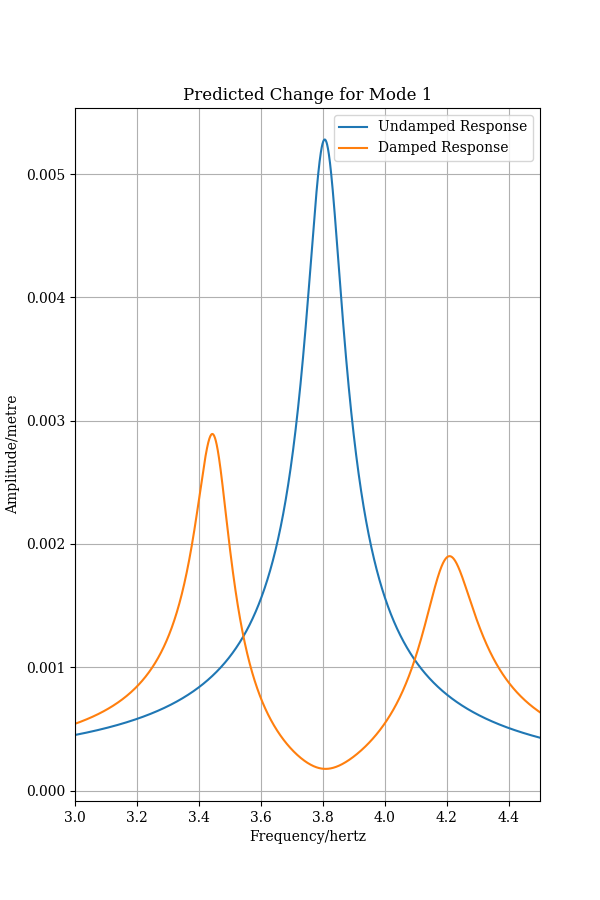
\includegraphics[width=.95\textwidth]{m1.png}
    \vspace{-14pt}
    \caption{Mode 1 - Floor 3}
    \end{subfigure}%
    \begin{subfigure}[b]{.4\textwidth}
    \centering
    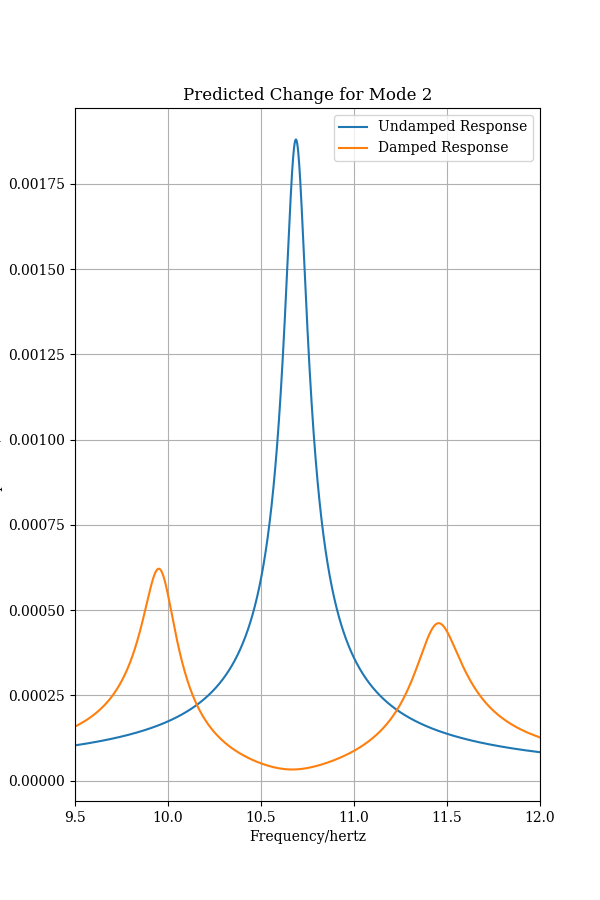
\includegraphics[width=.95\textwidth]{m2.png}
    \vspace{-14pt}
    \caption{Mode 2 - Floor 1}
    \end{subfigure}%
    \begin{subfigure}[b]{.4\textwidth}
    \centering
    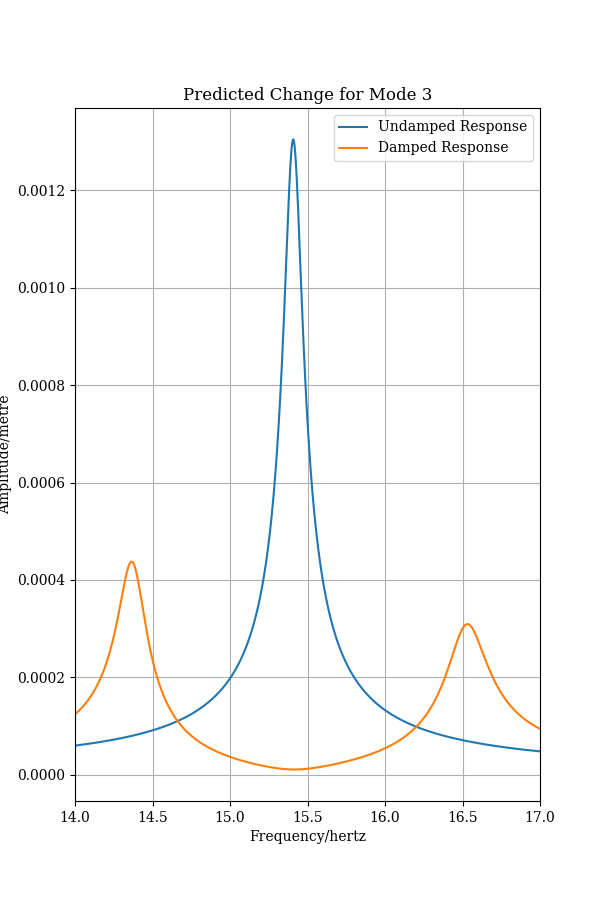
\includegraphics[width=.95\textwidth]{m3.png}
    \vspace{-14pt}
    \caption{Mode 3 - Floor 2}
    \end{subfigure}%
    }\\
    \vspace{-14pt}
    \caption{Numerical Simulation of the structure with individually tuned mass dampers}
\end{figure}

\vspace{-14pt}
\subsection{Predictions}
\vspace{-14pt}

From the results of these numerical simulations we can expect to see a reduction in the resonant response of the structure. It can also be observed
that the response splits into two smaller peaks above and below the resonant frequency.

Another prediction made is that invividually tuned mass dampers can be superimposed as the active frequencies of the tuned mass dampers are
far enough apart that they should not interact with each other.

\vspace{-14pt}
\section{Experimental Results}
\vspace{-14pt}

\begin{figure}[H]
    \centering
    \makebox[\textwidth][c]{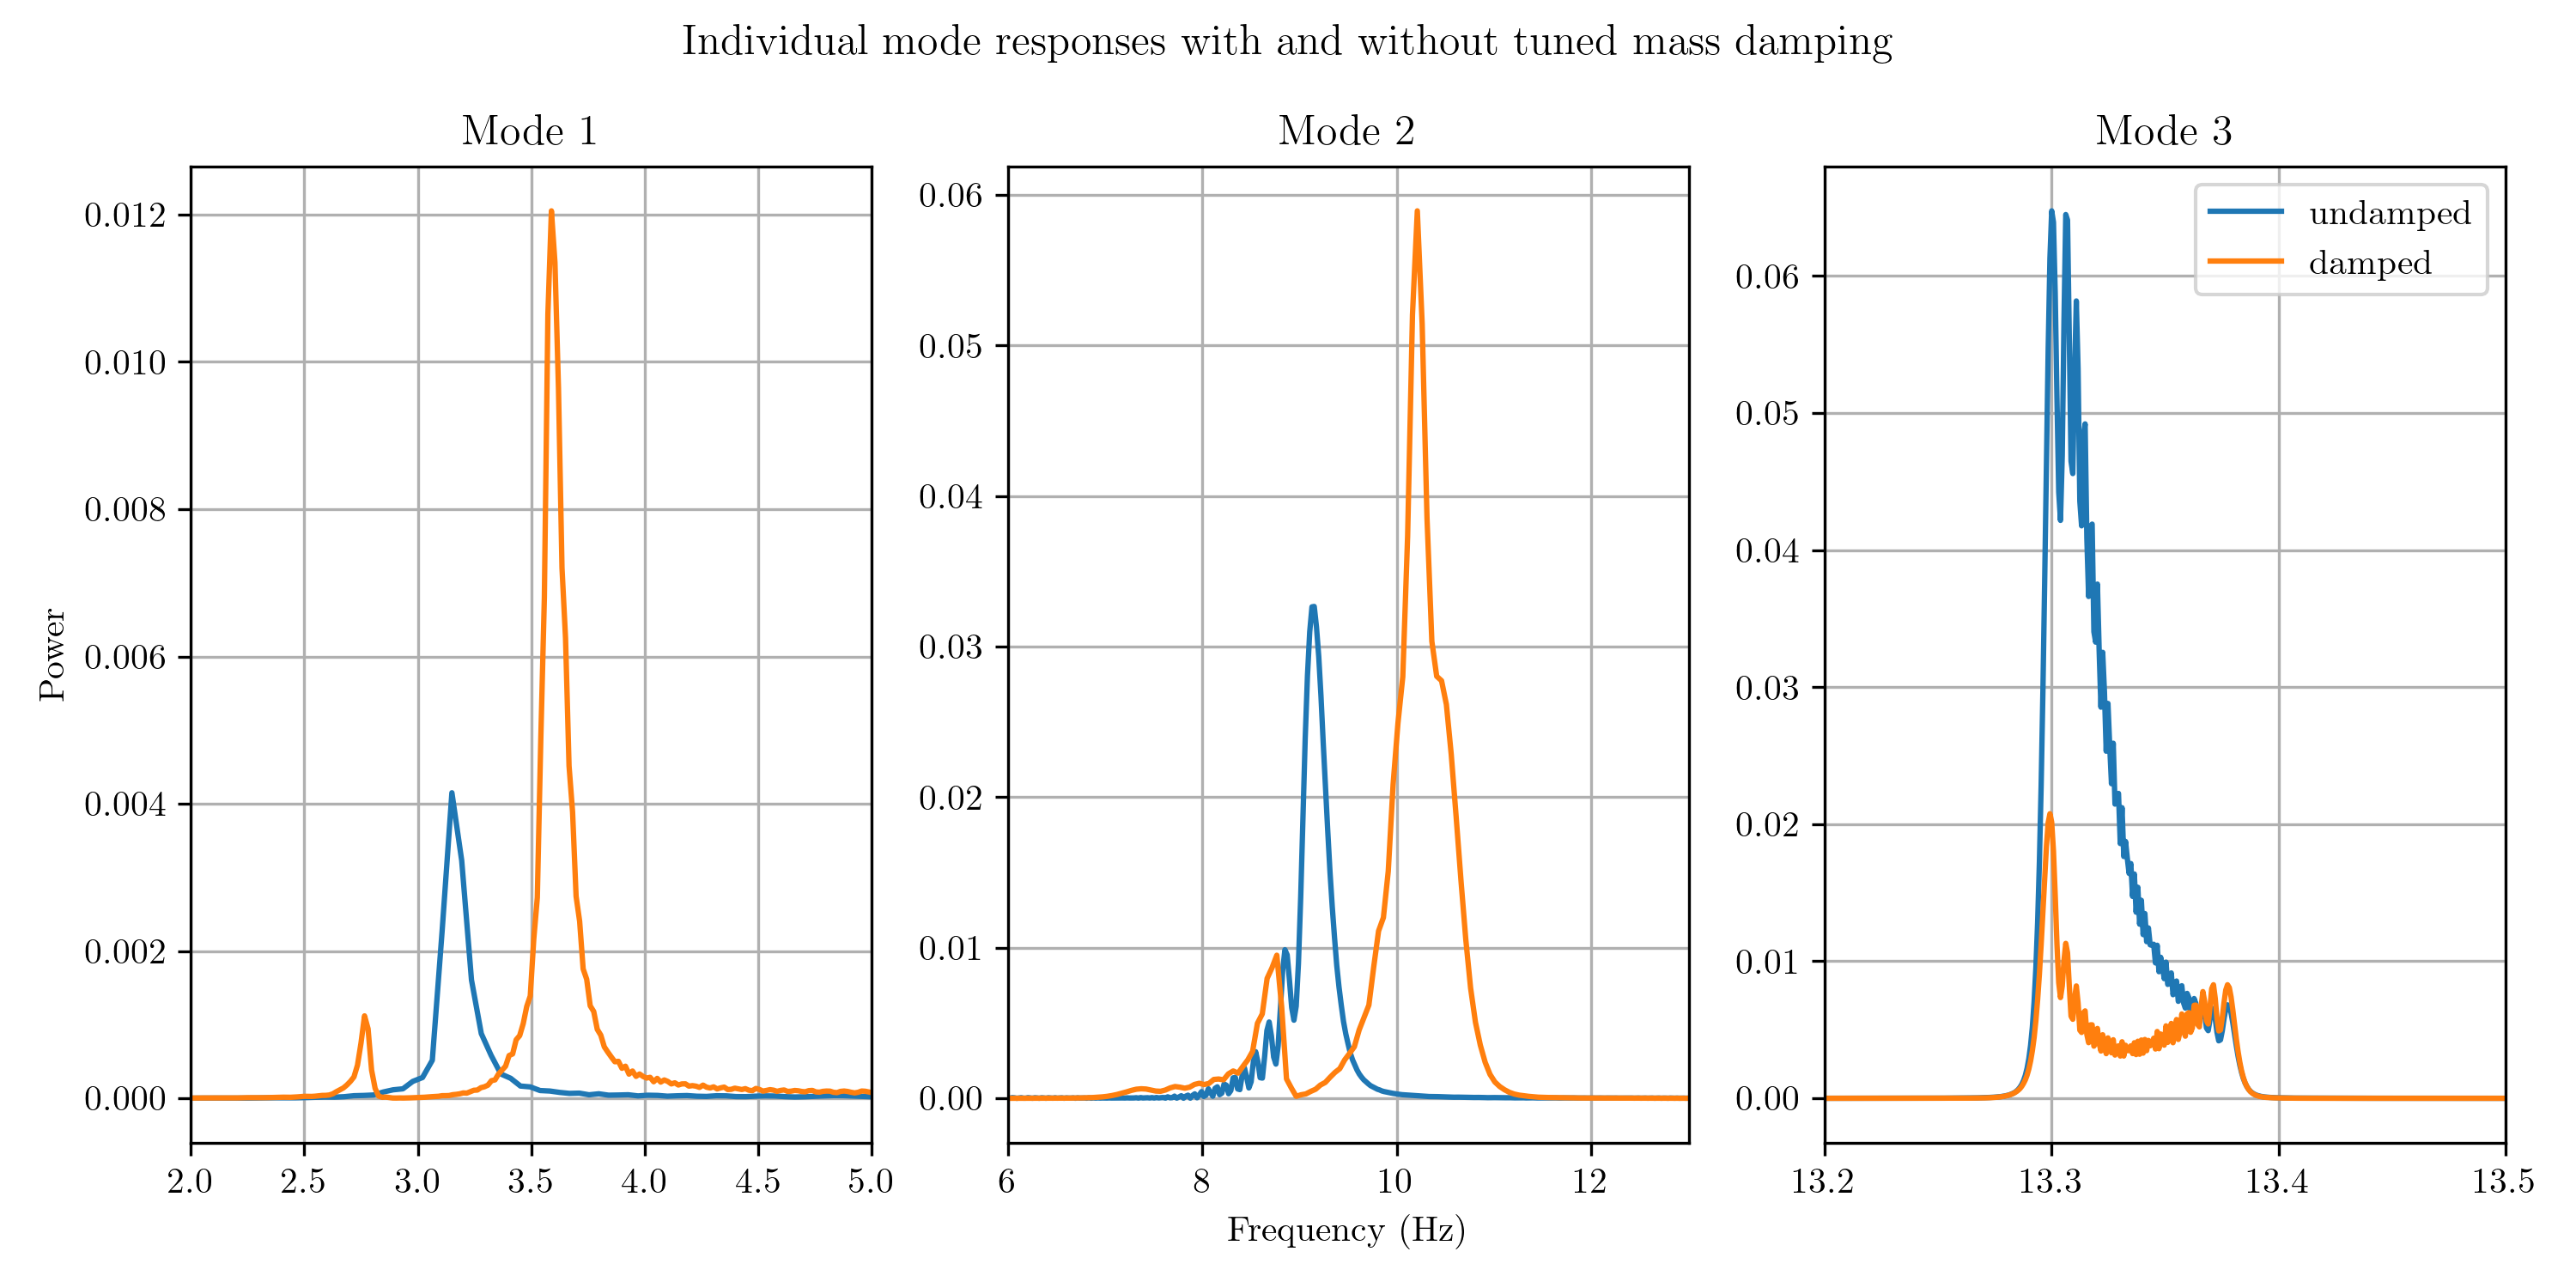
\includegraphics[width=1.2\textwidth]{modes.png}}
    \vspace{-14pt}
    \caption{\label{fig:modes} Harmonic responses of each node before and after the addition of a single tuned damper to that node}
\end{figure}

\begin{figure}[H]
    \makebox[\textwidth][c]{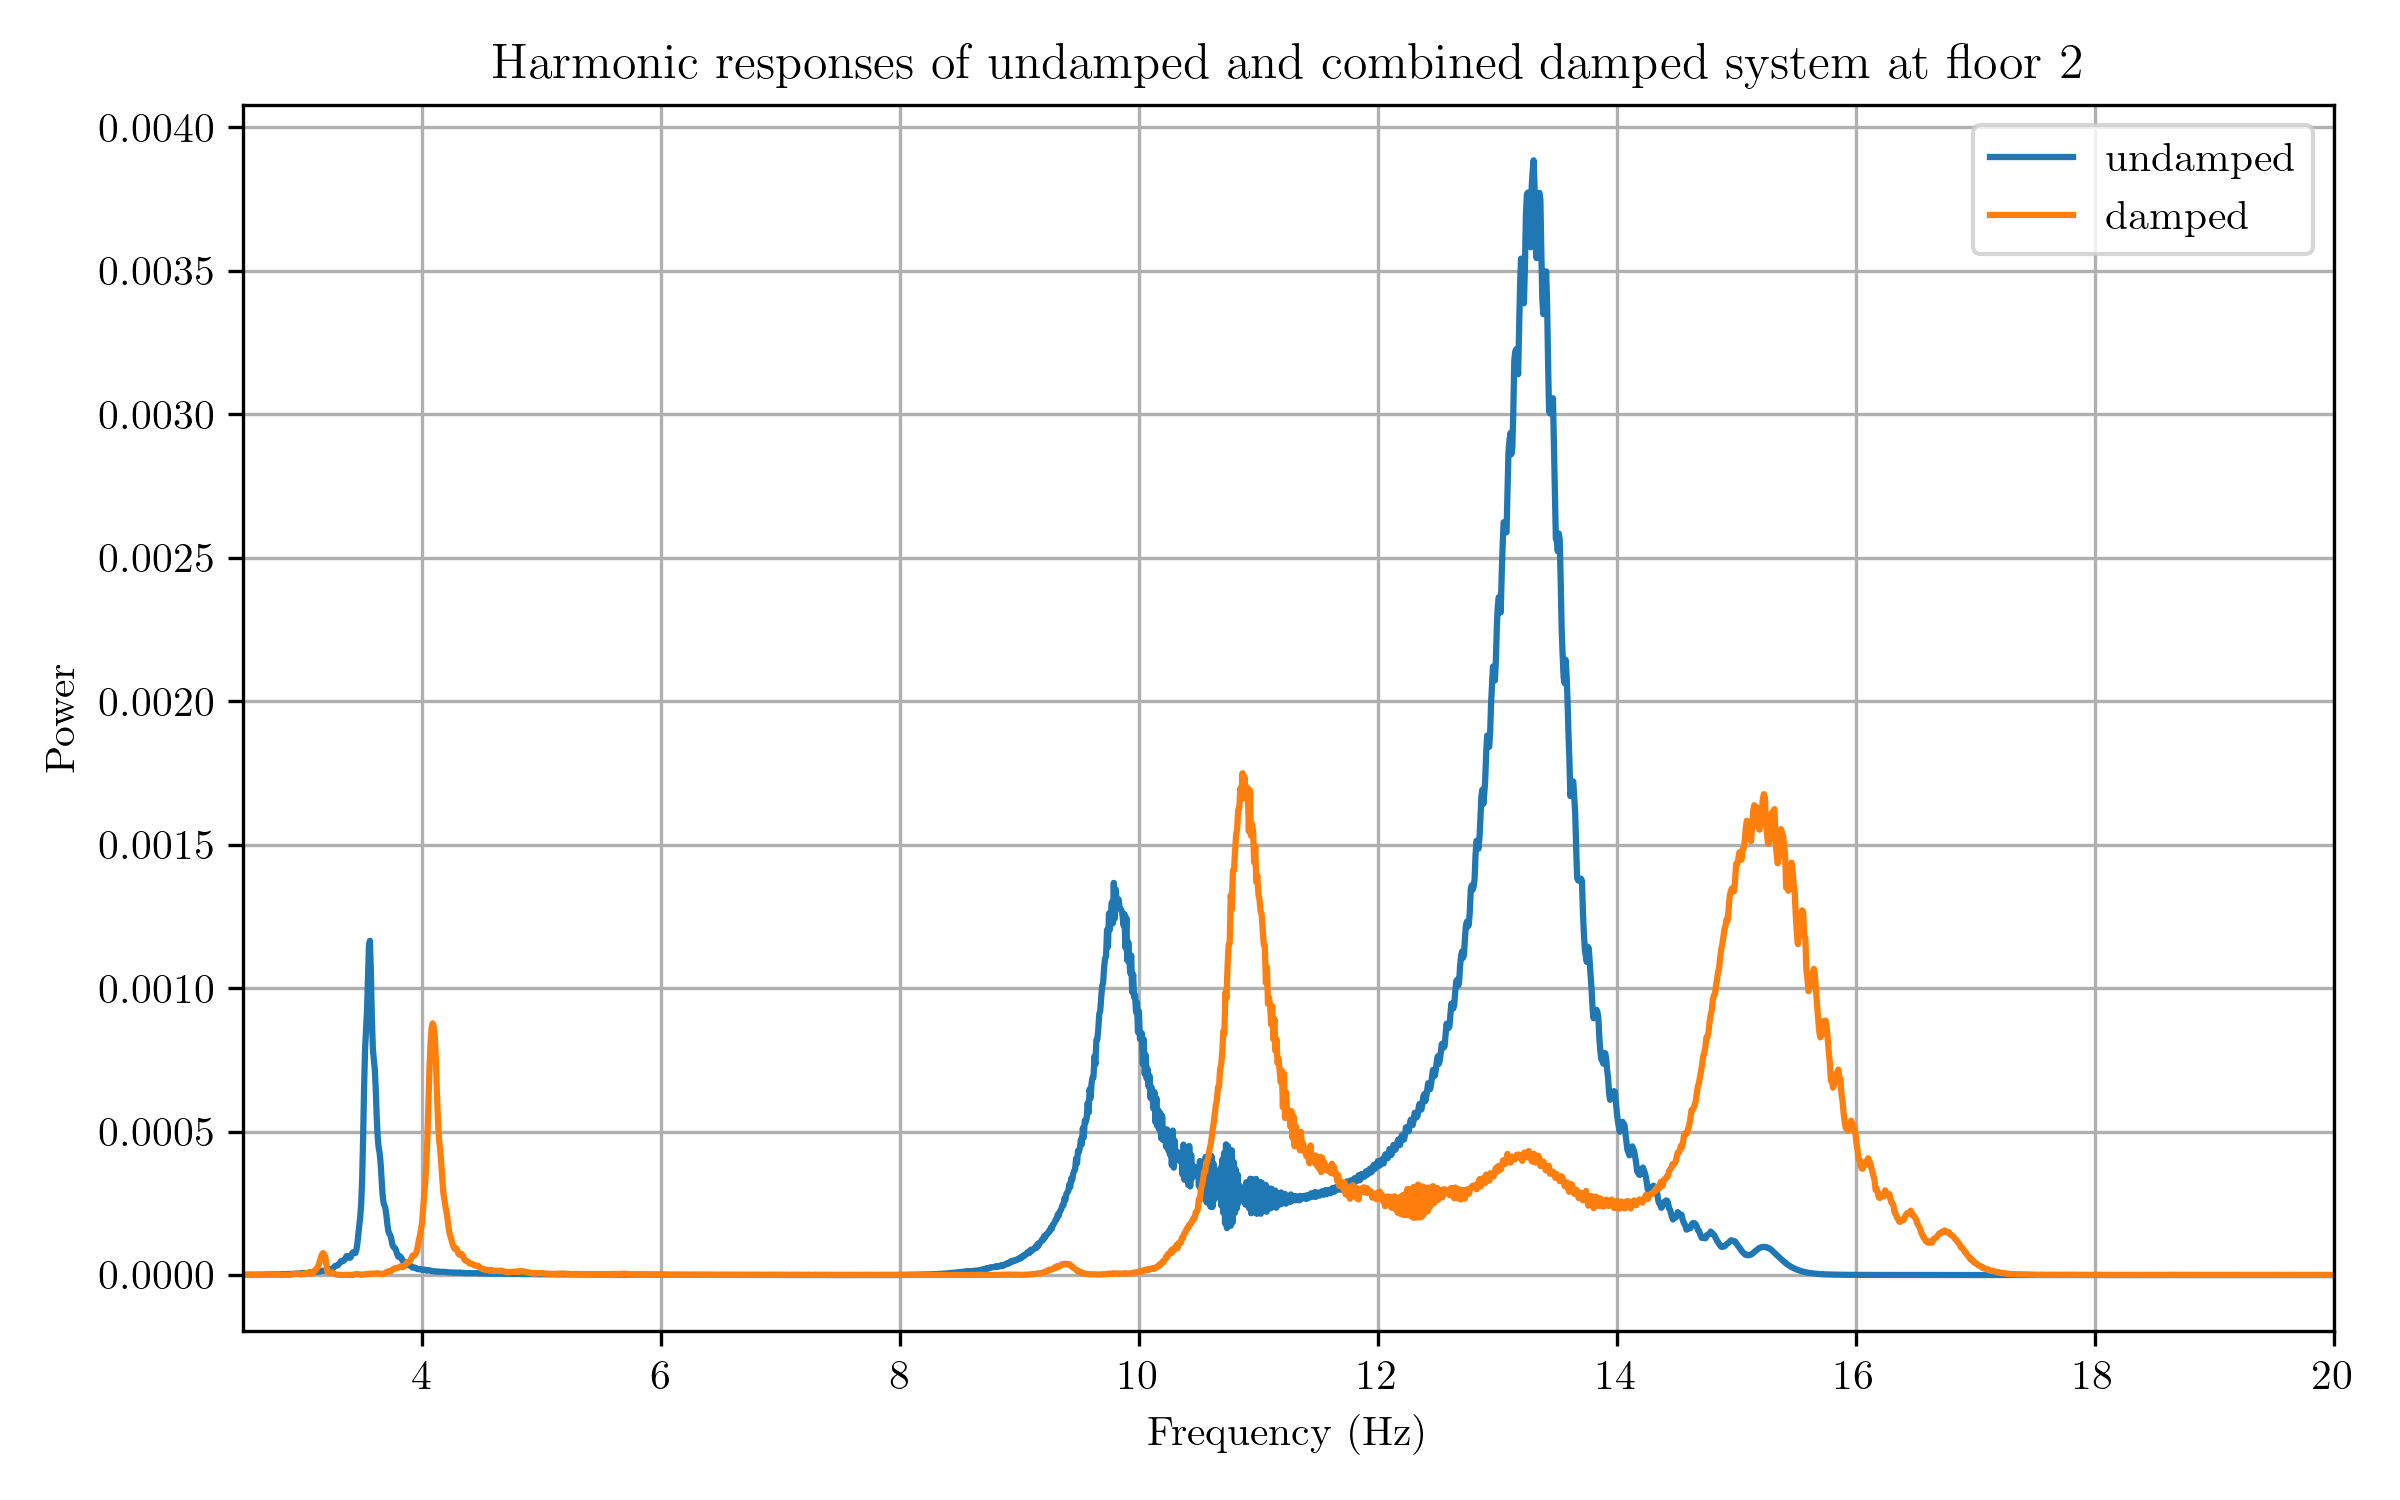
\includegraphics[width=1\textwidth]{combined_full_sweep.png}}
    \vspace{-14pt}
    \caption{\label{fig:combined_full_sweep} Harmonic response of structure before and after the addition of 3 tuned dampers at floor 2}
\end{figure}

\vspace{-24pt}
\section{Discussion}
\vspace{-16pt}

%interpret results and comment on anomalies


Figure \ref{fig:modes} shows the resonant response of each mode before and after the addition of a tuned mass damper.
In all cases the response at the original resonant frequencies has been reduced by the addition of the tuned mass damper. It can also be seen that the
response slightly above and below the resonant frequency increases. This is the predicted peak splitting.

\vspace{-8pt}

Modes 1 and 2 show an increased resonant response at the peak above the original resonant frequency.
This is likely due to The damping of the masses is very small as the air friction is negligible. 
This means that the two residual resonant responses are much higher than they would be if the absorbers had damping.

\vspace{-8pt}

The split peaks in the damped response are also highly asymetrical which suggests that the tuned mass dampers are not tuned to the resonant frequency of the structure.
This is due to our tuning method as the length of the cantilever was only tuned to the nearest 5mm.
This was done to reduce the time taken to tune the dampers as the tuning method was already very time consuming.

\vspace{-8pt}

Figure \ref{fig:combined_full_sweep} shows all resonant responses of the structure before and after the addition of the 3 individually tuned mass dampers.
Modes 2 and 3 show some interference as their split peaks overlap at about 12Hz. This was also qualitively observed by simultaneous vibration of the dampers.

\vspace{-20pt}

\subsection{Improvements}

\vspace{-16pt}

The tuning method used to tune the tuned mass dampers was not optimal and could be improved.
The damped response was highly sensitive to the length of the cantilever and so using callipers instead of a ruler would provide more accurate tuning.
Increasing the mass of the tuned mass dampers would help decrease the sensitivity of the response to changes of the length.

Tuning the damping factor would significantly reduce the response. This could be done in our case 
by adding plates of varying areas to the masses to increase the damping due to air resistance.
A better method would be to use a viscous damper which can be adjusted to tune an optimal damping coefficient.
Techniques such as gradient decent and genetic algorithms can be used to find multiple optimal parameters for simultaneous tuned mass dampers.

\vspace{-20pt}
\section{Conclusion}
\vspace{-16pt}

From the experimental data gathered it can be concluded that tuned mass dampers can be used to reduce the amplitude of resonant responses into two
smaller responses above and below the undamped resonant frequency.
However, tuning such dampers to the correct resonant frequency of the structure is not trivial and requires a large amount of experimentation.
This is due to high sensitivity of the response to changes in stiffness and in this case an untuned damping factor.

\end{document}
